% !TEX encoding = UTF-8
% !TEX TS-program = pdflatex
% !TEX root = ../tesi.tex

%**************************************************************
\chapter{Ricerca e sperimentazione}
\label{cap:ricerca-sperimentazione}
%**************************************************************

\intro{In questo capitolo viene descritto il processo di ricerca e sperimentazione di una soluzione efficace per l'implementazione dell'\acrshort{sso} nativo}\\

%**************************************************************
\section{Configurazione dello stato iniziale}

Avendo familiarità con Ubuntu ho, inizialmente, verificato che il pacchetto del server di FreeIPA fosse presente: ho presto appreso che esso era discontinuo sulle ultime versioni del sistema operativo.

Così, ho deciso di optare per \acrshort{centos} Stream 9, ultima versione disponibile, per l'ottima compatibilità con FreeIPA e la migliore usabilità in ambienti server.

A questo punto, con l'aiuto del team di \myAzienda, ho configurato \acrshort{lxc} sulla mia macchina Ubuntu 22.04 \acrfull{lts}.

Tramite il comando \texttt{lxc-create -t download -n ipa-server}, ho creato un nuovo container con il nome di \emph{ipa-server} indicando di voler scaricare il template dalla lista di quelli disponibili, dalla quale ho scelto l'immagine di \acrshort{centos} Stream 9 (\autoref{fig:lxc-template}).

Dopo la creazione della macchina ho lanciato i comandi \texttt{lxc-start ipa-server} e \texttt{lxc-console ipa-server}, rispettivamente per avviare il container e per accedere al relativo terminale.


Dopo aver configurato il container per il server ed aver eseguito l'aggiornamento dei pacchetti con il comando \texttt{yum update}, sono passato all'installazione del server di FreeIPA, disponibile su quella release con il pacchetto \emph{freeipa-server}.


Al mio arrivo negli uffici di \myAzienda, l'azienda aveva già configurato per me un account sulla loro piattaforma di testing, \emph{test.monokee.com}, utilizzando come e-mail il mio indirizzo istituzionale e garantendomi l'accesso a tutte le risorse della piattaforma, oltre che alla documentazione aziendale.

Inoltre, avevano predisposto sull'intranet aziendale, tramite Proxmox, delle macchine virtuali \acrshort{centos} e \acrshort{rhel} pronte all'uso (\autoref{fig:proxmox}).

\begin{figure}[H] 
    \centering 
    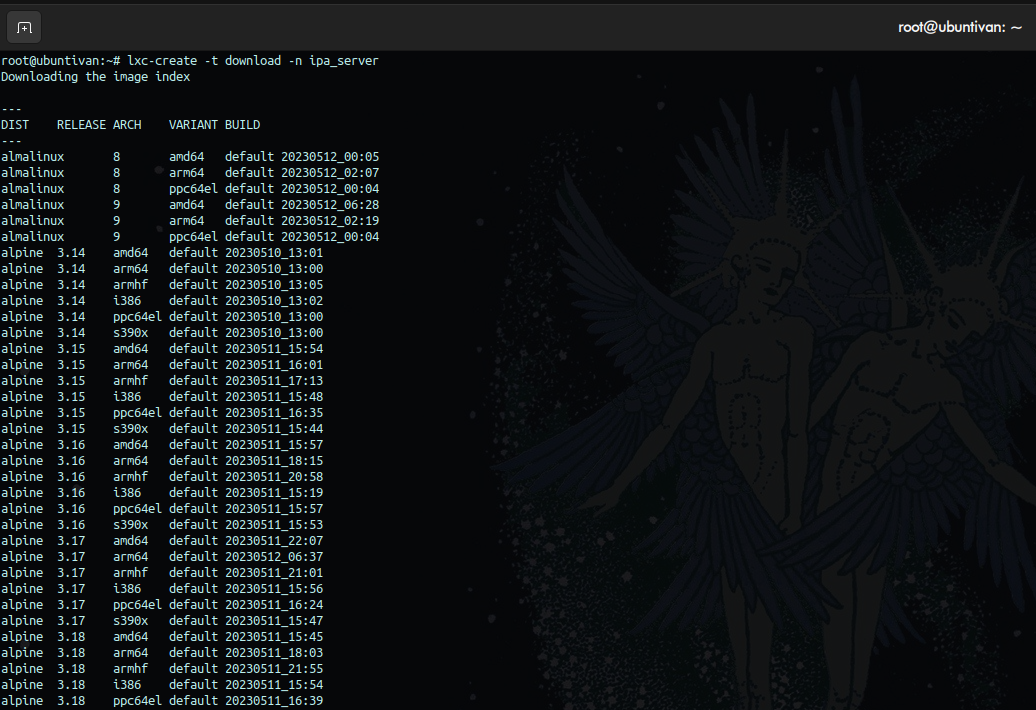
\includegraphics[width=\columnwidth]{lxc-templates} 
    \caption{Vista parziale del template download di LXC}
    \label{fig:lxc-template}
\end{figure}

\begin{figure}[H] 
    \centering 
    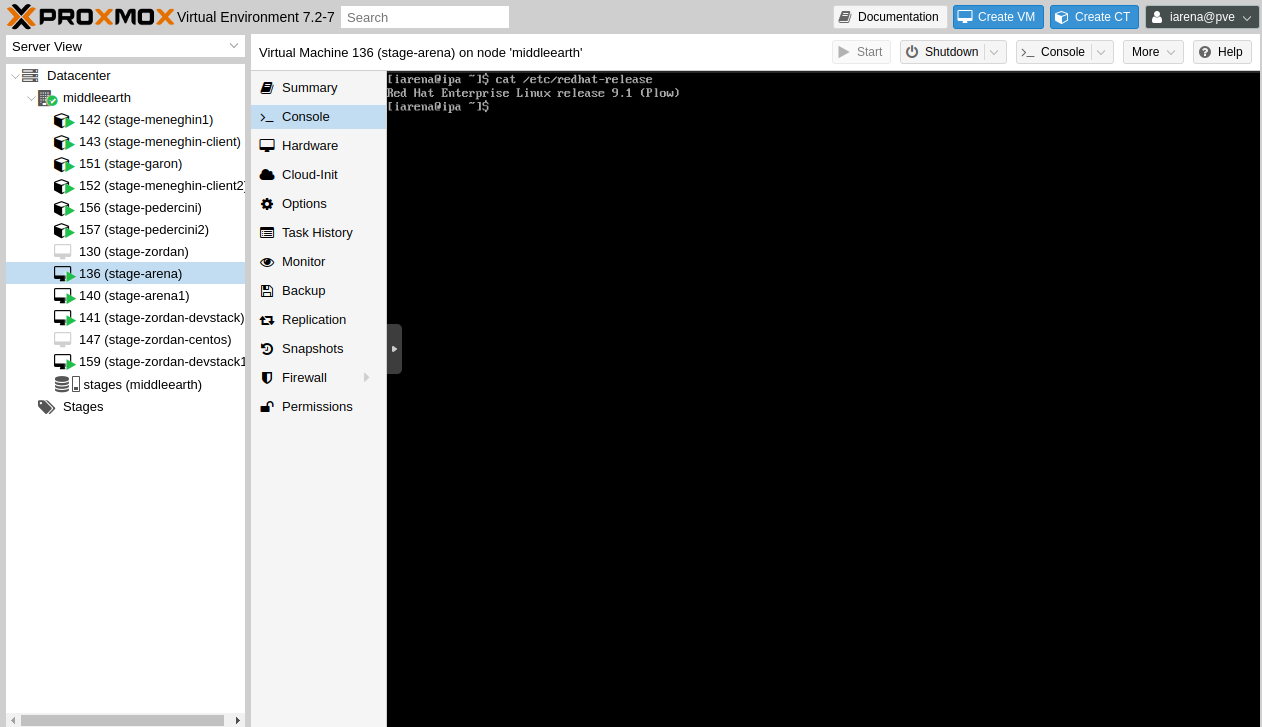
\includegraphics[width=\columnwidth]{proxmox} 
    \caption{Schermata di Proxmox con VM avviata}
    \label{fig:proxmox}
\end{figure}
\section{Linux Pluggable Authentication Modules}
\label{sec:tecnologie-strumenti}

La prima idea che ho avuto per integrare l'\acrshort{sso} di Monokee via \acrshort{ssh} sul container \acrshort{centos} che ho predisposto è stata quella di creare un nuovo modulo \acrshort{pam}. Ciò perché, studiando i file presenti al percorso \texttt{/etc/pam.d/} ho trovato il file \texttt{sshd}, che stabilisce i moduli da utilizzare per autenticazione, autorizzazione, sessione e gestione della password. In un primo momento mi sono concentrato sulla parte di autenticazione, controllando il file di configurazione \texttt{common-auth}, incluso in \texttt{/etc/pam.d/sshd}, che rappresenta l'autenticazione predefinita di UNIX (con password memorizzata localmente). 

Tuttavia, l'installazione di FreeIPA sovrascrive il parametro \texttt{UsePam yes} del file \texttt{/etc/ssh/sshd\_config} anteponendo dei parametri relativi a Kerberos, in modo da potersi autenticare con la password dell'utente FreeIPA specificato nel prefisso della macchina nel comando di \acrshort{ssh}.

La mia idea era, dunque, quella di rimuovere questi parametri e tornare all'autenticazione via \acrshort{pam}, sostituendo però il modulo predefinito con uno creato appositamente per l'\acrshort{sso} di Monokee.

Il problema restava quello del riconoscimento dell'utente ma avevo già pensato a diversi modi in cui poterlo risolvere, così ho deciso di proseguire e sperimentare con lo sviluppo di un modulo \acrshort{pam} di test, per verificare la fattibilità della mia intuizione.

\subsection{Sviluppo del modulo PAM}
Dapprima, ho deciso di sviluppare una semplice applicazione \acrshort{pam}-aware\cite{site:pam-app}, ovvero compatibile con Linux \acrshort{pam}, utilizzando il linguaggio C e facendo riferimento alla documentazione trovata\cite{site:writing-pam-application}\cite{site:understanding-pam}\cite{site:pam-configuration}\cite{site:linux-man-online}.  

Successivamente, ho sviluppato il modulo \acrshort{pam} di prova\cite{site:pam-module}\cite{site:pam-module-oidc} e l'ho impostato come metodo di autenticazione per l'\acrshort{ssh} con il seguente procedimento\cite{site:writing-pam-module}: prima di tutto, ho modificato il file di configurazione \texttt{/etc/ssh/sshd\_conf} disattivando il parametro \texttt{Set PasswordAuthentication} ed attivando il parametro \texttt{Set Use\acrshort{pam}}; in seguito, ho modificato il file di configurazione dei moduli \acrshort{pam} da utilizzare per il servizio \acrshort{ssh}, \texttt{/etc/pam.d/sshd}, commentando tutte le righe che facevano riferimento all'autenticazione ed inserendo una riga con il nome del modulo di prova che ho sviluppato, etichettato come \texttt{auth  sufficient}, indicando che era sufficiente ottenere esito positivo da tale modulo per autenticarsi con successo. 

\section{FreeIPA Identity Provider}

Dato che la soluzione con il modulo \acrshort{pam} si è rivelata essere più impegnativa del previsto, ho deciso di provare a configurare l'\acrshort{sso} con Monokee da FreeIPA. 

Navigando nell'interfaccia web del software, infatti, ho notato che nella sezione \textit{Authentication} > \textit{Identity Provider Servers} era possibile definire un \acrshort{idp} che utilizzasse \acrshort{oauth2} 2.0 come protocollo di autenticazione\cite{site:freeipa-docs}.

A questo punto, con l'aiuto del team, e, in particolare, del \acrfull{cto} di \myAzienda, mi sono spostato sull'infrastruttura di testing di Monokee per configurare un'applicazione \acrshort{oauth2} da poter utilizzare come Identity Provider per FreeIPA.

\section{Configurazione Monokee}
All'interno dell'ambiente di test di Monokee, tramite l'interfaccia web, ho creato una nuova applicazione \acrshort{oauth2}\cite{site:oauth-flow} \autoref{fig:monokee-oauth} ed un nuovo \acrshort{oidc} provider \autoref{fig:monokee-oidc}, che fornisse gli end-point per l'autenticazione via \acrshort{oidc}\cite{site:monokee-docs}.


\begin{figure}[H] 
    \centering 
    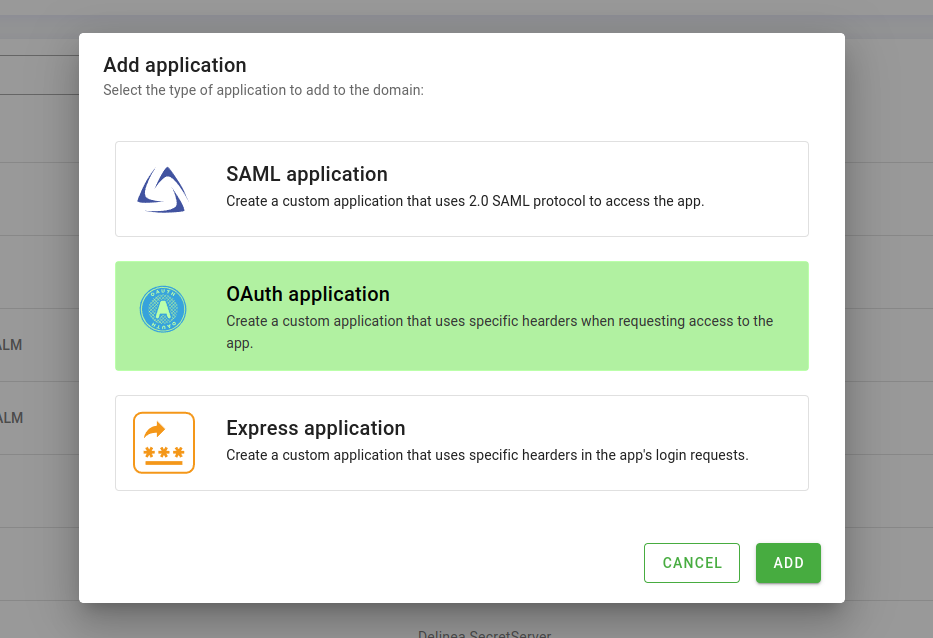
\includegraphics[width=0.7\columnwidth]{monokee-oauth-app} 
    \caption{Schermata di creazione app OAuth2 da Monokee}
    \label{fig:monokee-oauth}
\end{figure}

\begin{figure}[H] 
    \centering 
    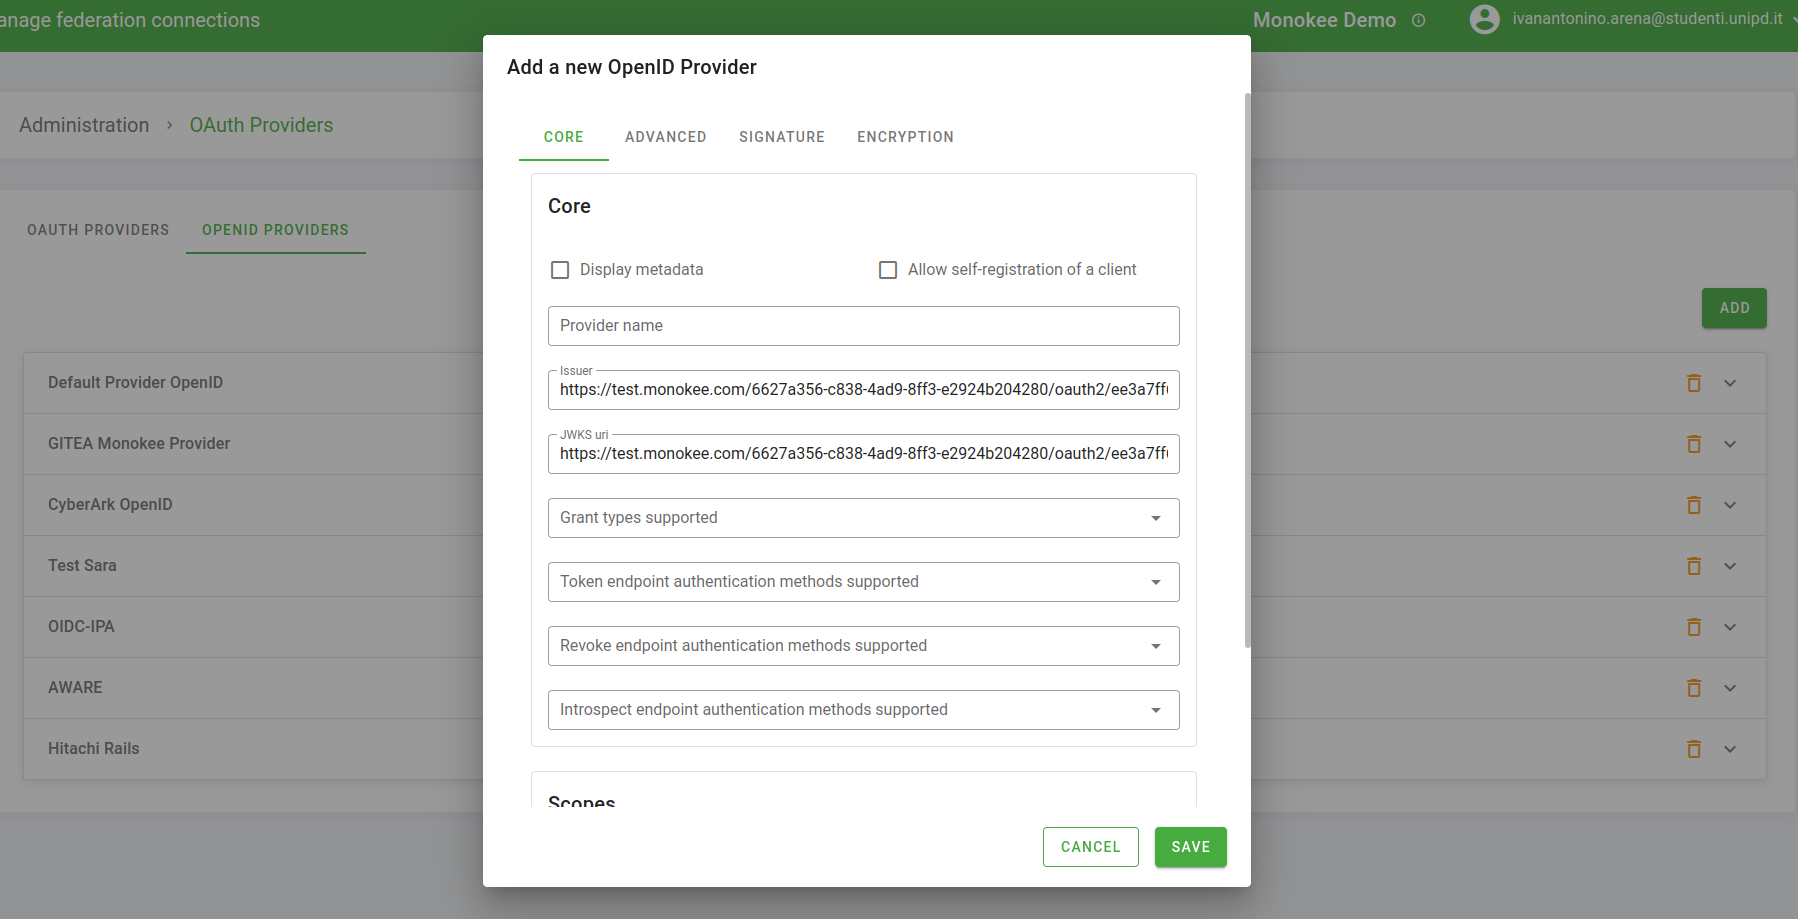
\includegraphics[width=0.7\columnwidth]{monokee-oidc} 
    \caption{Schermata di creazione OpenID provider da Monokee}
    \label{fig:monokee-oidc}
\end{figure}

\section{Configurazione FreeIPA}
Da FreeIPA, ho proceduto a configurare un nuovo Identity Provider server, tramite la sezione della \acrfull{gui} di cui sopra, inserendo tutte i metadati richiesti, facendo riferimento all'applicazione \acrshort{oauth2} creata su Monokee e agli end-point forniti dall'OpenID provider configurato precedentemente.

Successivamente, ho creato un utente FreeIPA che utilizzasse come unico metodo di autenticazione quella tramite Identity Provider esterno (\emph{External \acrshort{idp}}), scegliendo Monokee come \acrshort{idp} e come identificatore il mio indirizzo e-mail istituzionale, già associato al mio account Monokee, per poter eseguire l'accesso via \acrshort{sso} con le mie credenziali\cite{site:using-ext-idp-idm}.  

Configurata correttamente l'infrastruttura di autenticazione sia su Monokee che su FreeIPA, ho proceduto a verificarne il funzionamento seguendo le indicazioni della documentazione relativa: dapprima, ho generato un file per l'autenticazione tramite canale FAST con il comando \texttt{kinit -n -c ./fast.ccache}; successivamente, ho richiesto l'autenticazione anonima tramite PKINIT con il comando \texttt{kinit -T ./fast.ccache monokee1}; a questo punto, viene eseguito il flusso di \acrshort{oidc} e viene mostrato un URL al quale autenticarsi tramite \acrshort{sso} di Monokee; ad autenticazione eseguita, basta tornare sul terminale e premere invio per completare l'autenticazione.

Per verificare la corretta autenticazione ho poi lanciato il comando \texttt{klist}, che mostra i ticket Kerberos richiesti, e controllato che l'utente attuale fosse lo stesso con cui volevo autenticarmi e che il ticket fosse valido (\autoref{fig:ipa-cli}).  

\begin{figure}[H] 
    \centering 
    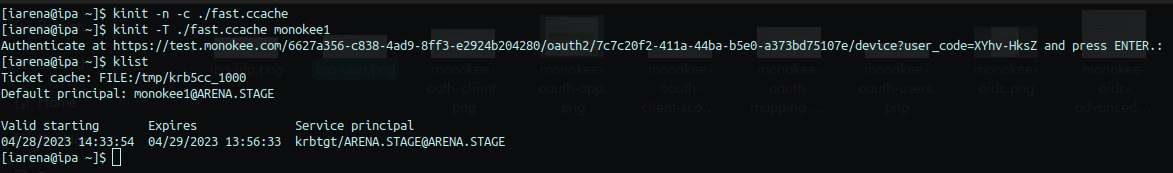
\includegraphics[width=\columnwidth]{ipa-cli} 
    \caption{Autenticazione con Monokee SSO tramite FreeIPA da CLI}
    \label{fig:ipa-cli}
\end{figure}


\section{Problematiche riscontrate}

Durante l'integrazione dell'\acrshort{sso} tramite FreeIPA, nonché già dal processo di configurazione dello stesso, ho riscontrato numerose problematiche.

In primis, a rendere il processo più faticoso del previsto, è stata la mancanza di una  documentazione esaustiva e di informazioni utili in rete in merito alla risoluzione degli errori, dovuta probabilmente alla userbase di FreeIPA, che, benché tale servizio sia lo standard in ambito \acrshort{iam}, è alquanto ridotta.

In secondo luogo, mi sono imbattuto errori di inconsistenza piuttosto limitanti tra i registri di FreeIPA e quelli di sistema, riscontrati anche da altri utenti in rete\cite{site:redhat-bugzilla} \cite{site:freeipa-issue} \cite{site:freeipa-users-1} \cite{site:freeipa-users-2} \cite{site:freeipa-users-3} \cite{site:centos-forums}, oltre che difetti di compatibilità della piattaforma con alcune versioni di \acrshort{centos} e \acrshort{rhel}.

Infine, l'autenticazione di FreeIPA tramite Monokee \acrshort{sso} non riesce a sovrascrivere quella di UNIX quando si vuole raggiungere una macchina tramite \acrshort{ssh} su un utente Monokee già configurato sul server. Tuttavia, ho raggiunto il monte ore stabilito prima di poter arrivare ad una soluzione per questa problematica; l'attuale implementazione, dunque, comprende la possibilità di accedere al proprio ambiente Monokee tramite \acrshort{sso} da una certa macchina client unicamente se si è autenticati all'interno di essa con un utente locale di qualunque tipologia.

\section{Documentazione}

\myAzienda ha richiesto la redazione di una guida che illustrasse il processo di configurazione del server FreeIPA e dei sistemi di Monokee per l'integrazione del \acrshort{sso} sulle macchine UNIX, per fornire una base documentativa per facilitare le future progressioni e sperimentazioni relative. Seguendo le indicazioni dell'azienda, ho utilizzato il formato Markdown, versionando il codice sul repository GitHub aziendale fornitomi dalla stessa\cite{site:docs}. La documentazione consta di un singolo file Markdown di 188 righe, completo di comandi, codice ed immagini esplicative.



\section{Sviluppi futuri}
A partire dai risultati che ho ottenuto durante l'attività di stage, gli sviluppi futuri possibili sono molteplici.

Innanzitutto, comincerei con il risolvere il problema legati all'accesso alle macchine con il server di FreeIPA installato tramite \acrshort{ssh} su un utente di FreeIPA, e, dunque, per mezzo del \acrshrot{sso} di Monokee. L'\acrshort{sso}, difatti, viene bypassato e viene richiesta la password dell'utente, la quale, di fatto, non esiste perché non è utilizzata da FreeIPA sugli utenti da autenticare con Monokee. 

Dunque, andrei a verificare le impostazioni attive nei file di configurazione di \acrshort{ssh}, come \texttt{/etc/ssh/sshd\_config}.
\\ \\
Risolto questo problema e avendo, quindi, una macchina a cui è possibile accedere tramite \acrshort{ssh} direttamente con un utente Monokee, il prossimo passo potrebbe essere quello di predisporre delle macchine server con le risorse dell'azienda e fornirne l'accesso 
direttamente da Monokee, utilizzando un servizio come Apache Guacamole.

In questo modo, un utente Monokee privilegiato potrebbe accedere a delle macchine server gestire accessi, privilegi ed altro, oppure, nel caso di un utente subordinato, accedere a delle macchine client, gestite da quella server.